
\section{Available Data}
There are two suitable datasets for this task, which will both be used to train the sentiment analysis tool on.
\subsection{EmoBank}
This dataset is the most important one for this project, as it contains 10,000 English sentences covering multiple genres, all annotated with their own VAD values \cite{emoBank}.

\begin{center}
\begin{tabular}{ |c|c| } 
 \hline
  Sentence Type & Frequency \\ 
 \hline         
 News Headlines & 1192 \\
 Blogs & 1336 \\
 Essays & 1135 \\
 Fiction & 2753 \\
 Letters & 1413 \\
Newspapers & 1314 \\
 Travel Guides & 919\\
 \hline
 Sum & 10062 \\
 \hline
\end{tabular}
\end{center}

This dataset contains VAD values for each piece of text from both writer and the reader of the text, but due to the findings in \cite{emoBank} only the values given by the reader will be used, as it is concluded that this perspective has higher emotionality and therefore they should be easier to train with.

Initial prototyping using this dataset shows that it is easy to implement into machine learning tools, but there is an issue with the distribution of data, as shown in Figure \ref{emoBank:dist}. When the sentences are split into buckets depending on their valence values, there is a very large disparity in the frequency of each bucket represented, meaning that training on this dataset leads to incorrect classification of test data.

\begin{figure}[h]
\caption{Graph showing the distribution of the valence of all the sentences in the EmoBank corpus, with 0 being very negative and 10 being very positive}
\centering
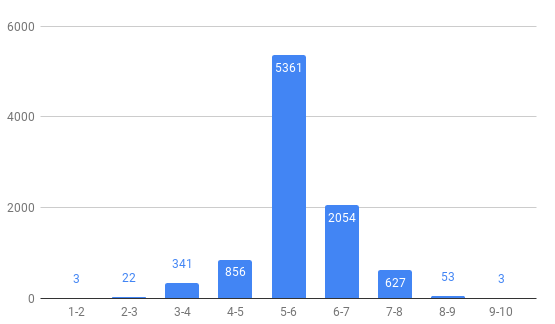
\includegraphics[scale=1.8]{./LitReview/images/valence-frequency-bucket-graph.png}
\label{emoBank:dist}
\end{figure}

Another issue with this dataset is that because it is not big enough, it is occasionally incorrectly classifying words as negative which shouldn't be. An example of this is where it repeatedly classifies "Italy" as being a negative word. This is due to the dataset containing a letter from someone who had an unpleasant holiday in Italy. To counteract this issue, I plan on using more data in conjunction with this dataset so hopefully this situation will become less prevalent.

So far in prototyping the sentiment analysis tool on this has only been trying to predict the valence of the words. Trying other classification systems has not been done yet, and is currently in production. 

\pagebreak

\subsection{Affective Ratings for Words}
To increase the range of data to train with, a dataset that contains VAD values for almost 14,000 English words\cite{wordsData} is also being incorporated, and can help balance out unnecessarily strongly weighted words by reclassifying them into a more appropriate emotional state. The issue with having only the individual words rated with VAD values means that the context in which the words are used can be lost, so this is a case where using a bag-of-words method for splitting up the sentences may not be the most appropriate.

\begin{figure}[h]
\caption{Graph showing the distribution of the valence of all the sentences in the EmoBank corpus, with 0 being very negative and 10 being very positive}
\centering
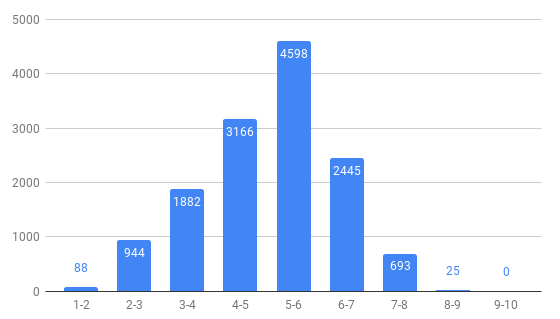
\includegraphics[scale=1.9]{./LitReview/images/words-valence-buckets.png}
\label{words:dist}
\end{figure}
